\section{Motivation}
Diese Ausarbeitung wird für das Fach Softwarearchitektur an der technischen Hochschule Rosenheim geschrieben.
Das Ziel ist es OpenHAB, ein Heimautomatisierungs-Tool, aus praktischer und technischer Sicht zu untersuchen. Dabei liegt der Fokus vor allem auf der Softwarearchitektur von OpenHAB. 

\section{Was ist OpenHAB}
OpenHAB ist eine technologie-unabhängige Open-Source-Automatisierungssoftware für Smart-Homes.
Sie wurde von Kai Kreuzer 2010 erstmals initiiert und wird mittlerweile durch die Community weiterentwickelt. OpenHAB ist in Java geschrieben und aktuell in der Version 2.4 erhältlich.\\
\\
Auf der offiziellen Website von OpenHAB \url{https://www.openhab.org/} sind drei klare Hauptziele definiert, die diese Software erreichen soll. Ein Ziel ist die Plattformunabhängigkeit. Somit kann OpenHAB sowohl auf Linux, MacOS oder Windows betrieben werden. Auch das hosten mit Docker oder einem Raspberry Pi wird unterstützt.\\
Weiterhin soll es durch die Plugin-Architektur  möglich sein, fast jedes Gerät zu integrieren.
Es werden über 200 Technologien und mehrere tausende verschiedene Geräte unterstützt.\\
Das dritte Ziel weißt auf die vielen verschiedenen Automatisierungsmöglichkeiten hin, die OpenHAB zu bieten hat. Dabei werden Auslöser, Aktionen, Skripte und auch Voice-Kontrolle genannt.


\section{Datenintegriertät und Sicherheit}
\url{https://www.openhab.org/docs/installation/security.html}
\begin{itemize}
	\item Through the command line console, which is done through SSH and thus always authenticated and encrypted. You will find all details about this in the Console documentation.
	\item Through HTTP(S), which we will look at in the following.
\end{itemize}

\section{OpenHAB aus technischer Sicht}
In diesem Kapitel sind die grundlegenden Komponenten, die OpenHAB verwendet, tabellarisch dargestellt. Anschließend wird detaillierter auf die einzelnen Elemente eingegangen.

\begin{longtable}{| p{2cm} | p{13cm}|}
	\hline
	\textbf{Konzept} & \textbf{Beschreibung} \\
	\hline \hline
	\centering Bindings & sind die openHAB-Komponenten, die die Schnittstelle zur elektronischen Interaktion mit Geräten bereitstellt.  \\
	\hline
	\centering Things & sind die erste von openHAB (Software) generierte Darstellung von Geräten. \\
	\hline
	\centering Channels & sind die openHAB (Software)-Verbindung zwischen "`Dingen"' und "`Gegenständen"'. \\
	\hline
	\centering Items & sind die von openHAB (Software) generierte Darstellung von Informationen über die Geräte.\\
	\hline
	\centering Rules & führen automatische Aktionen durch (in einfachster Form: wenn "`dies"' passiert, wird openHAB "`das"' tun).\\
	\hline
	\centering Sitemaps & ist die von openHAB (Software) generierte Benutzeroberfläche (Website), die Informationen präsentiert und Interaktionen ermöglicht.\\
	\hline
	\caption{OpenHAB Komponenten}
	\label{table:openhub-components}
\end{longtable}

\subsection{Bindings}
\begin{itemize}
	\item Typische Bindings
	\item Screenshot?
	\item Geräteerkennung
\end{itemize}

\subsection{Things}

\subsection{Channels}

\subsection{Items}
\begin{itemize}
	\item Items können gruppiert werden
\end{itemize}
\begin{lstlisting}[language=java,firstnumber=1,caption=Item-Gruppierung Beispiel,label=lst:group-items]
	Group groundFloor
	Switch kitchenLight (groundFloor)
	Switch livingroomLight (groundFloor)
\end{lstlisting}

\subsection{Rules}


\subsection{Sitemaps}

\subsection{Api}
\url{https://www.openhab.org/docs/configuration/restdocs.html}
\begin{itemize}
	\item Item ausschalten
	\item Eine List von allen Items, Sitemaps ausgeben lassen
	\item \dots
\end{itemize}

\section{Verwendung von OpenHAB}
\subsection{Integration der Big Player}
\begin{itemize}
	\item Amazon Alexa und Echo Dot Integration möglich
	\begin{itemize}
		\item \url{https://www.openhab.org/docs/ecosystem/alexa/}
		\item \url{https://www.openhab.org/addons/bindings/amazonechocontrol/}
	\end{itemize}
	\item Google Home Integration möglich \url{https://www.openhab.org/docs/ecosystem/google-assistant/}
\end{itemize}

\subsection{Beispiel Aufbau eines OpenHAB Smart-Homes}
\begin{itemize}
	\item OpenHAB auf Raspberry Pi 3/4 installiert
	\item Welche Geräte haben wir mit OpenHAB verbunden?
	\begin{itemize}
		\item Spotify
		\begin{itemize}
			\item Lautstärkeregler
			\item Aktueller Song Display
		\end{itemize}
		\item LG Smart TV
		\begin{itemize}
			\item Lautstärkeregler
			\item An- und ausschalten
			\item One-Way-Chat
		\end{itemize}
		\item Lampen
	\end{itemize}
	\item Wie haben wir die Geräte verbunden?
	\begin{itemize}
		\item \textbf{Verschiedene Binding:}
		\item Spotify Binding
		\item LG Smart TV Binding
	\end{itemize}
	\item Welche Rules haben wir angewendet und wofür?
	\item On the server the configuration is stored somewhere in userdata (/var/lib/openhab2 for apt-get installs).
	In an upgrade the userdata folder is preserved when using apt-get.
\end{itemize}
\begin{minipage}{\textwidth}
	\centering
	\captionsetup{type=figure}
	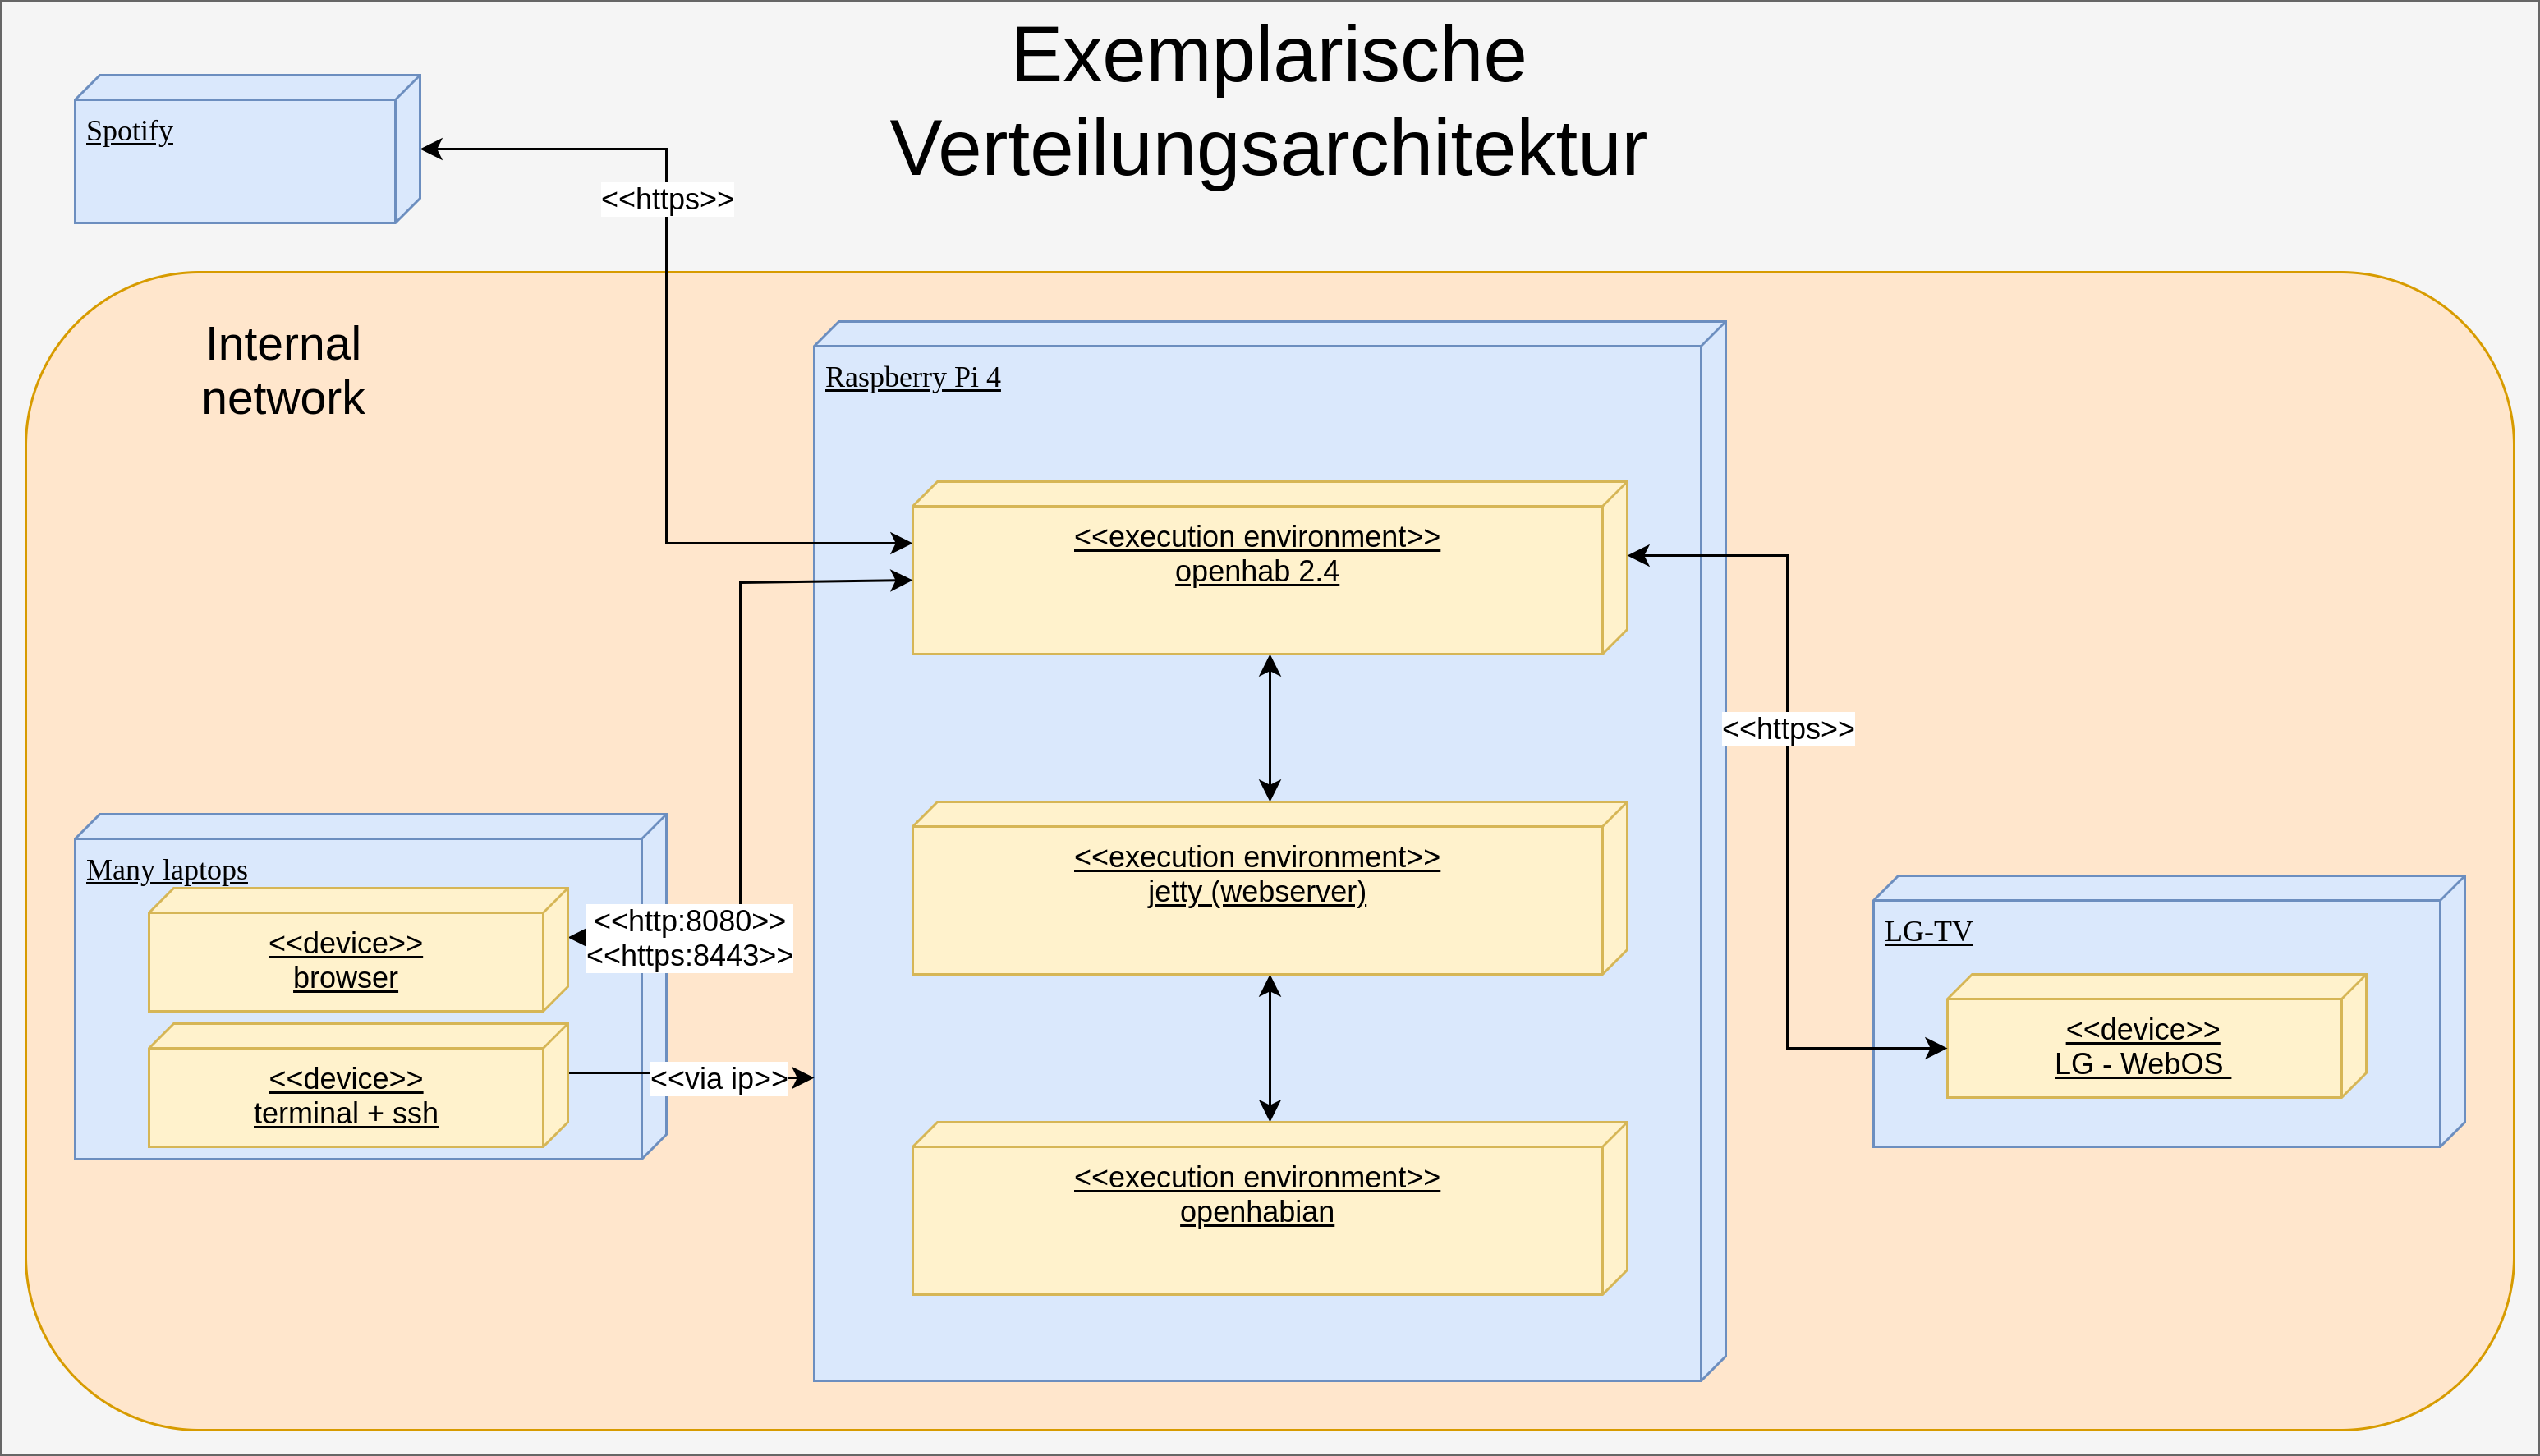
\includegraphics[width=1\textwidth]{\figdir/verteilungsarchitektur.png}
	\caption{Verteilungsarchitektur \label{fig:verteilungs-architektur}}
\end{minipage}

\section{Fazit}
\subsection{Stärken}
Some of openHAB's strengths are:

Its ability to integrate a multitude of other devices and systems. openHAB includes other home automation systems, (smart) devices and other technologies into a single solution
To provide a uniform user interface and a common approach to automation rules across the entire system, regardless of the number of manufacturers and sub-systems involved
Giving you the most flexible tool available to make almost any home automation wish come true; if you can think it, odds are that you can implement it with openHAB.
\subsection{Schwächen}
\textbf{Wollen wir das hier als SWOT Analyse aufziehen?}
\begin{itemize}
	\item Integration von USB-Geräten scheint eher kompliziert. Vor allem auf Raspberry Pi
	\item Serial Binding wird nicht angezeigt
	\begin{itemize}
		\item Mikrofon an Raspberry Pi oder anderes Geräte verbinden
		\item Input des Mikrofons über OpenHAB an ein Ausgabegerät, wie zum Beispiel eine Bluetooth Box, senden und abspielen
		\item Raspberry hat da auch für große Probleme bei der Geräteerkennung gesorgt - USB gerät wurde nicht im devices Verzeichnis aufgeführt und somit konnte auch keine Verbindung mit OpenHAB aufgebaut werden
		\item OpenHAB Serial Device Binding wurde auch nicht angezeigt, um Geräte darüber zu suchen
	\end{itemize}
	\item Doku ist schwer verständlich
	erste schritte klappen leicht, aber danach wird es schwierig
\end{itemize}

\section{Infos:}
\textbf{Ausgangslage}
Untersuchen Sie die Architektur und Features von OpenHAB und
schreiben Sie ein Beispielanwendung.
Mit myOpenHub existiert eine kostenlose Plattform die sie nutzen
können.

\textbf{Beantworten Sie dabei}
\begin{itemize}
 \item Aktueller Status des Projekts und  
 \item Integration der Big Player wie Alexa und Google Home
 \item Welche Tools und Konzepte und APIs gibt es
 \item Welche Deployment Modi und Betriebsmodi existieren
 \item Untersuchen Sie auch Aspekte wie Datenintegriertät und Sicherheit
\end{itemize}

\textbf{Unterlagen Linkes}
\begin{itemize}
	\item \url{https://www.myopenhab.org/}
	\item \url{https://www.openhab.org/}
	\item \url{https://jaxenter.de/openhab-2-4-78711}
\end{itemize}


\section{Vorlage mit Samples}

Einen Überblick findet man z.\,B.\ in \cite{Auer00:HTF}.

\begin{figure}[t]
	\centering
	
	\begin{subfigure}{0.45\linewidth}
		\centering
		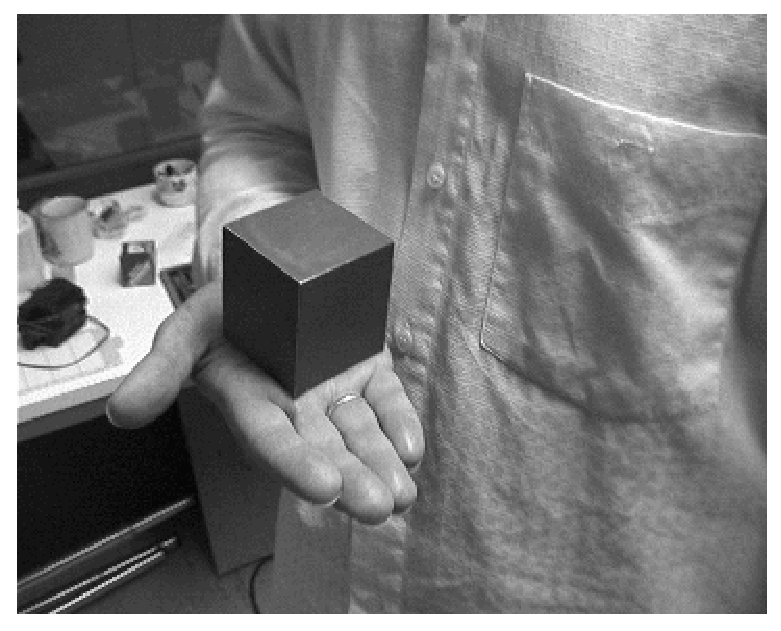
\includegraphics[width=\linewidth]{\figdir/handorig}
		\caption{Originalbild}
		\label{FIG:arexorig}
	\end{subfigure}
	%
	\begin{subfigure}{0.45\linewidth}
		\centering
		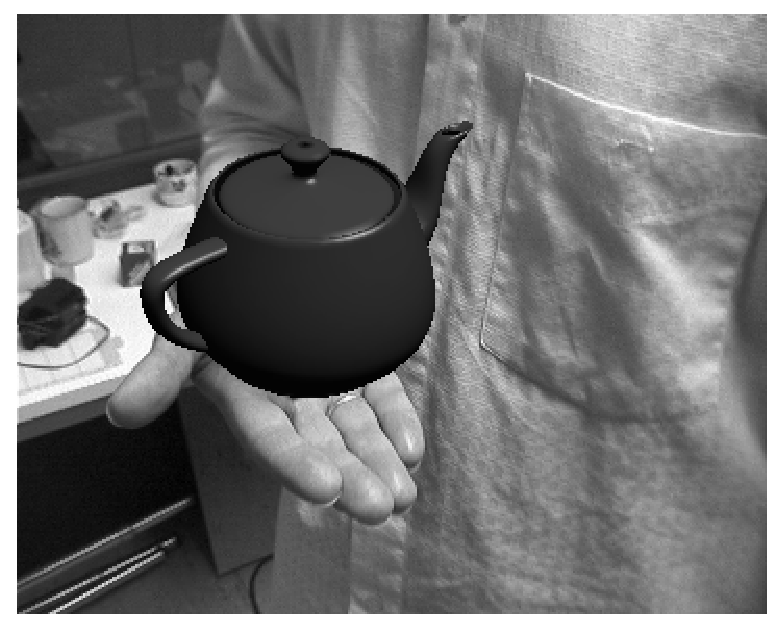
\includegraphics[width=\linewidth]{\figdir/handaug}
		\caption{erweitertes Bild}
		\label{FIG:arexaugm}
	\end{subfigure}
	%
	\caption[AR Beispiel]
	{Beispiel eines Augmented Reality Systems: es folgt eine Beschreibung (Bilder aus \cite{Schmidt01:PAO})}
	\label{FIG:arex}
\end{figure}

Ein Beispiel wird in Abb.\ \ref{FIG:arex} gezeigt.
Das verwendete Objekt ist in Abb.\ \ref{FIG:arexorig} dargestellt, das Ergebnis in Abb.\ \ref{FIG:arexaugm}.

Eine Formel
\begin{equation}
\label{eq:cvp:test}
f(x) = \frac{1}{3} x + 5, \quad x \in \real.
\end{equation}

Und noch eine:
\begin{equation}
\label{eq:cvp:matvec}
\bm{M}  = \bm{Ax} \pi, \quad \bm{A} \in \real^{2 \times 2}, \bm{x} \in \real^2.
\end{equation}

Tabelle \ref{t:CodebookOverview} gibt einen Überblick über XYZ.

\begin{table}[t]
	\centering\small
	%
% generated by TexTableGenerator.pl ((c) Florian Vogt)
% from file: /home/Jochen/data/dissdata/results/CodebookOverview.log
%
\begin{tabular}{l|ccc|cc}
\hline
\hline
                  \textbf{Sequence} &          ARTS &           wman &         stcams &         ARTVZ &        ARTSUZ \\ 
                 \textbf{\# Frames} &             190 &              40 &             400 &             270 &             190 \\ 
     \textbf{\# relative movements} &           17955 &             780 &           79800 &           36315 &           17955 \\ 
\textbf{\# movements after pre-sel.} &           14336 &             623 &           37915 &           21788 &           14343 \\ 
       \textbf{min.\ angle in seq.} &   0.233$^\circ$ &    5.95$^\circ$ &   0.154$^\circ$ & 0.00000171$^\circ$ &  0.0388$^\circ$ \\ 
       \textbf{max.\ angle in seq.} &    81.7$^\circ$ &     180$^\circ$ &    47.3$^\circ$ &    80.3$^\circ$ &    80.9$^\circ$ \\ 
\textbf{min.\ angle after pre-sel.} &    12.9$^\circ$ &    21.1$^\circ$ &    17.3$^\circ$ &    16.3$^\circ$ &    12.9$^\circ$ \\ 
\textbf{max.\ angle after pre-sel.} &    81.7$^\circ$ &     161$^\circ$ &    47.3$^\circ$ &    80.3$^\circ$ &    80.9$^\circ$ \\ \hline\hline
\end{tabular}

	\caption[Testtabelle]{Datenselektion für verschiedene Testdatensätze.}
	\label{t:CodebookOverview}
\end{table}


%%% Local Variables: 
%%% mode: latex
%%% TeX-master: "thesis.tex"
%%% End: 
